===================== TO THIS POINT =============

For $\beta \gg 1$ $\sigma(\beta N_t)\approx u(N_t)$, meaning
\begin{equation}
	\begin{split}
		\sum_{s_1,s_2,\dots s_L}u(N_L)
		p(s_{1},s_{2},\dots s_{L}|D,I) & = p(\sum_{t'=1}^Ls_{t'} \leq N_0+U_{0}|D,I)\\
		& = p(\text{no stockout at time L})
	\end{split}
\end{equation}
meaning
\begin{equation}
	p(\text{no stockout at time t})\approx\frac{\psi_{L}}{(H-L)k_{L}+\psi_{L}}
	\label{eq:d_rule1}
\end{equation}
This consequently means that
\begin{equation}
	U_0 = \bigg(\frac{\psi_{L}}{(H-L)k_{L}+\psi_{L}}\cdot 100 \% \text{ percentile of } \sum_{t'=1}^L s_{t'}\bigg)- N_0
	\label{eq:dec_rule}
\end{equation}


\begin{example}
	Consider the case of $N_0=27$, $L = 9$, $k_t=5$, $\psi_t=1000$ and $\sum_{t'=1}^{L-1}U_{t'-L}=0$. Figure \ref{fig:forecast_example} show the historical (blue), forecasted (green) and true future (orange) number of units that are removed from the stock. In this example, the number of units removed from the stock follows a Poisson distribution with a rate parameter of $\lambda= 3$ (unknown to the Robot). The Robot estimate the rate parameter using maximum likelihood viz $\hat{\lambda}= \frac{1}{N}\sum_{i=1}^{N}s_i=3.025$. The forecast then consist of sampling from a Poisson distribution with rate parameter $\hat{\lambda}$.
	\begin{figure}[H]
		\centering
		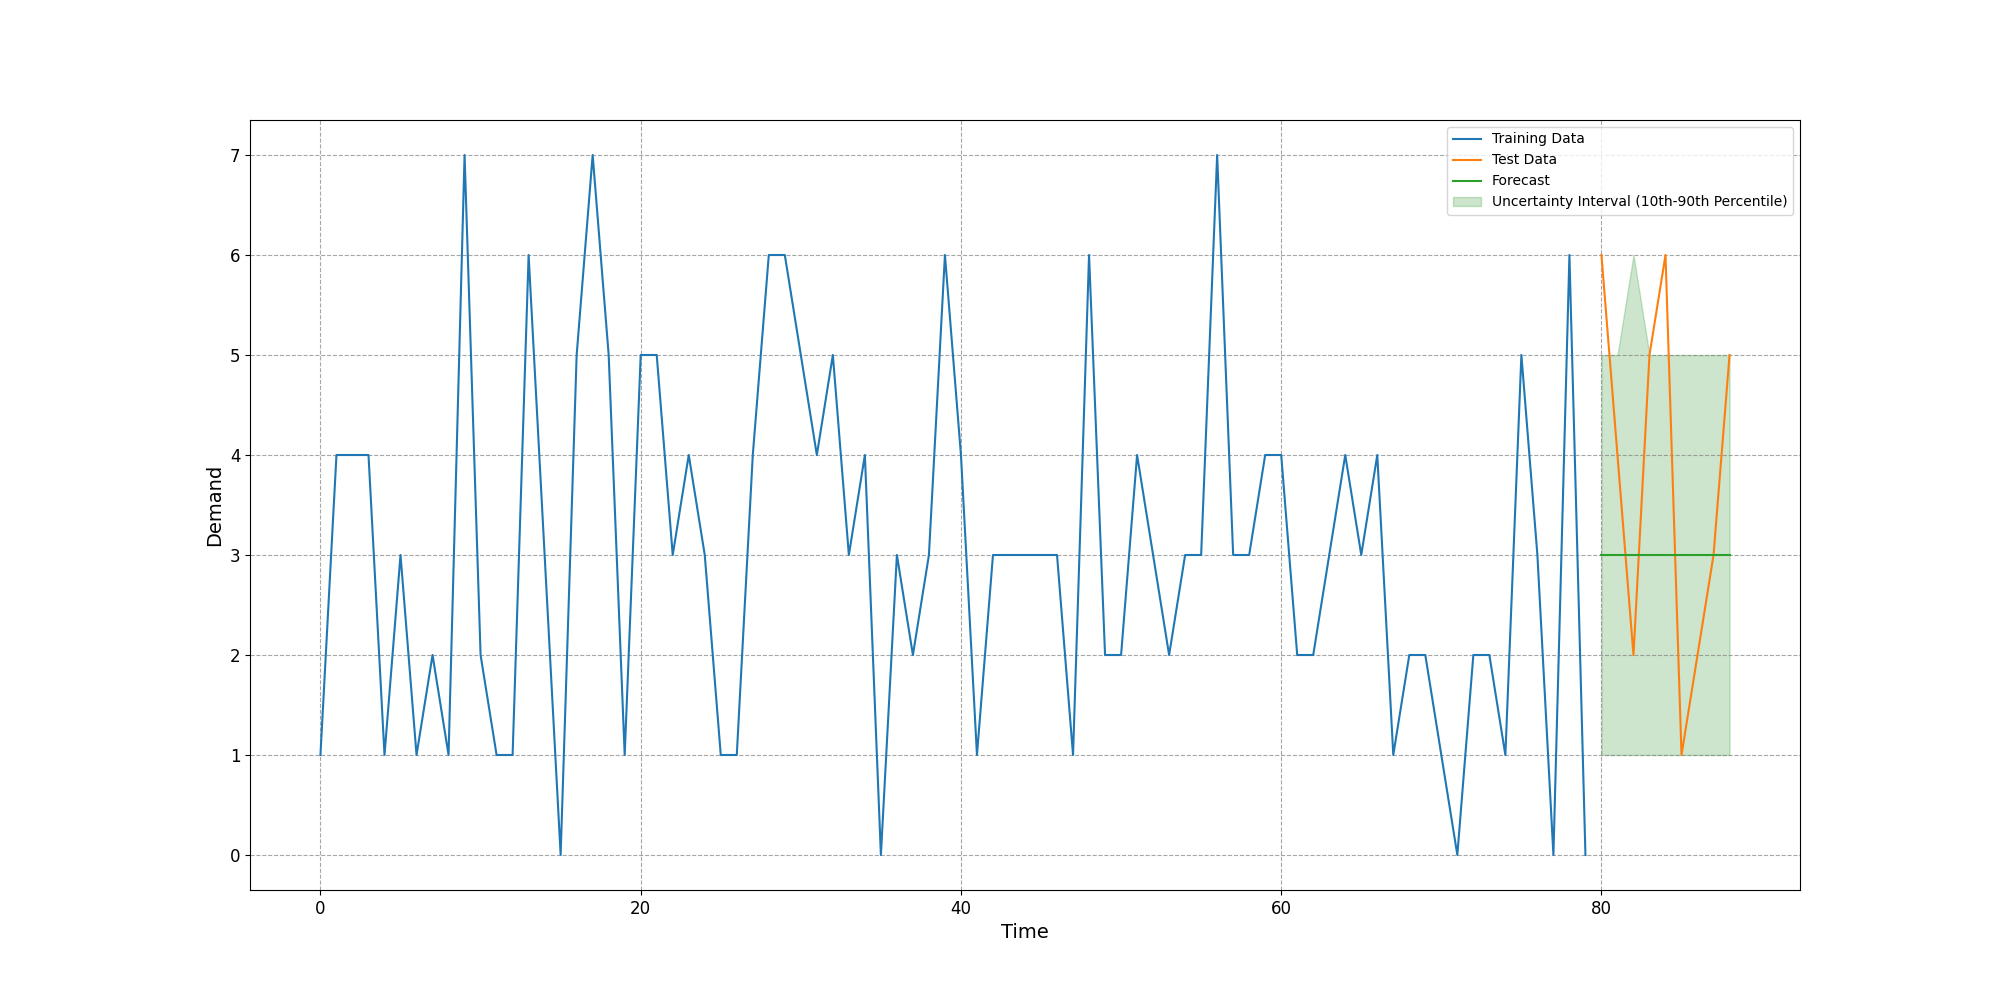
\includegraphics[width = 1\textwidth]{figures/forecast_example.png}
		\caption{Historical removal of units from stock (blue), forecasted removal from stock (green) and future removal from stock (orange).}
		\label{fig:forecast_example}
	\end{figure}
	Using the approach from section \ref{sec:1}, the Robot would make the decision
	
	\begin{equation}
		\begin{split}
			U_0^{(1)} &= \max\bigg(\sum_{t'=1}^{L}\hat{s}_{t'}-N_{0}-\sum_{t'=1}^{L-1}U_{t'-L},0\bigg)\\
			&=  \max(L\lambda-N_0,0)\\
			& = 0
		\end{split}
	\end{equation}
	Figure \ref{fig:demand_density} show the probability distribution of demand during the lead time. The median of the distribution is $L\lambda$, but it is clear there is a significant probability mass for $\sum_{i=1}^{L}s_i>L\lambda$. 
	
	\begin{figure}[H]
		\centering
		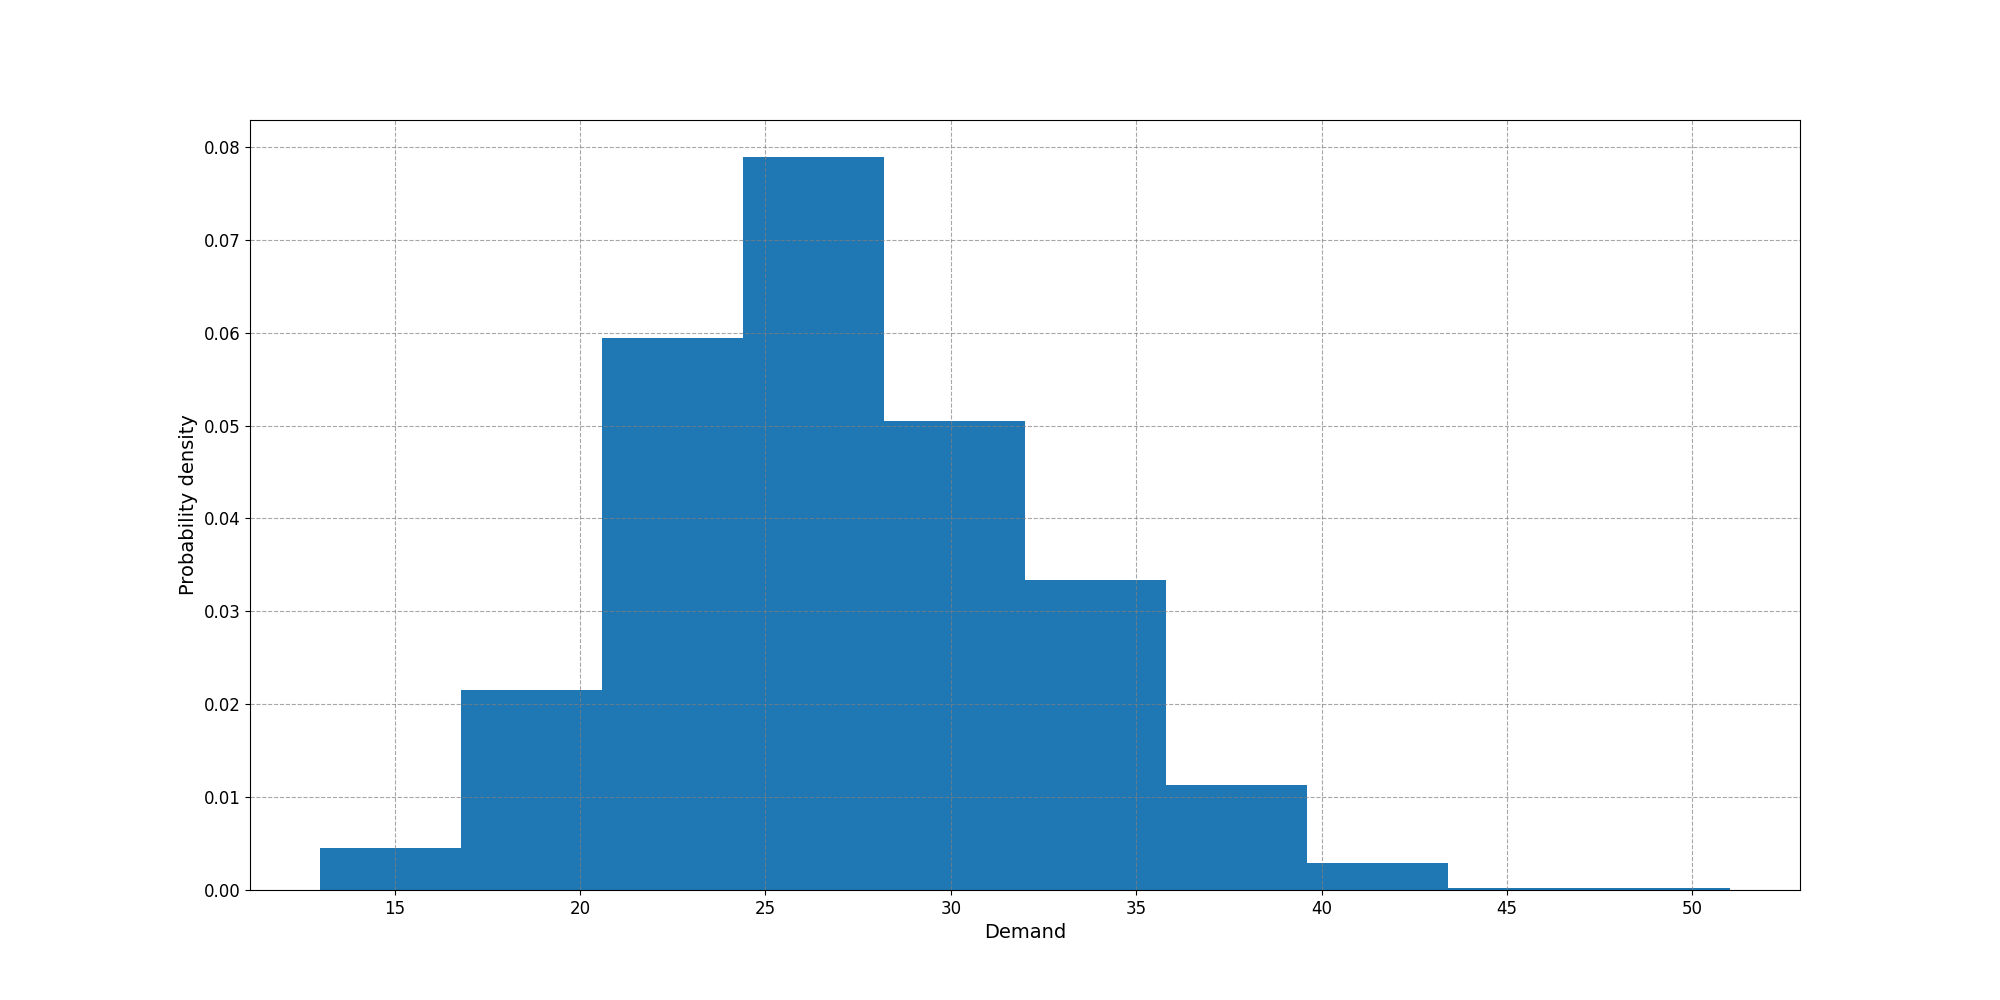
\includegraphics[width = 1\textwidth]{figures/demand_density.png}
		\caption{The distribution of $\sum_{i=1}^{L}s_i$.}
		\label{fig:demand_density}
	\end{figure}
	
	Using the approach from section \ref{sec:2} and in particular equation \eqref{eq:dec_rule}, the Robot would make the decision
	\begin{equation}
		U_0^{(2)}=9
	\end{equation}
	
	Figure \ref{fig:cost_function} show the cost function (blue) alongside the decisions $U_0^{(1)}$ (orange), $U_0^{(2)}$ (red) and the perfect decision in retrospective (brown). The blue curve, and consequently the red line, can be adjusted by adjusting $\psi_t$, meaning the penalty for under stocking. The figure illustrates that there can be a big difference between decision derived from the forecast without decision theory and the decision derived from the forecast using decision theory. 
	
	\begin{figure}[H]
		\centering
		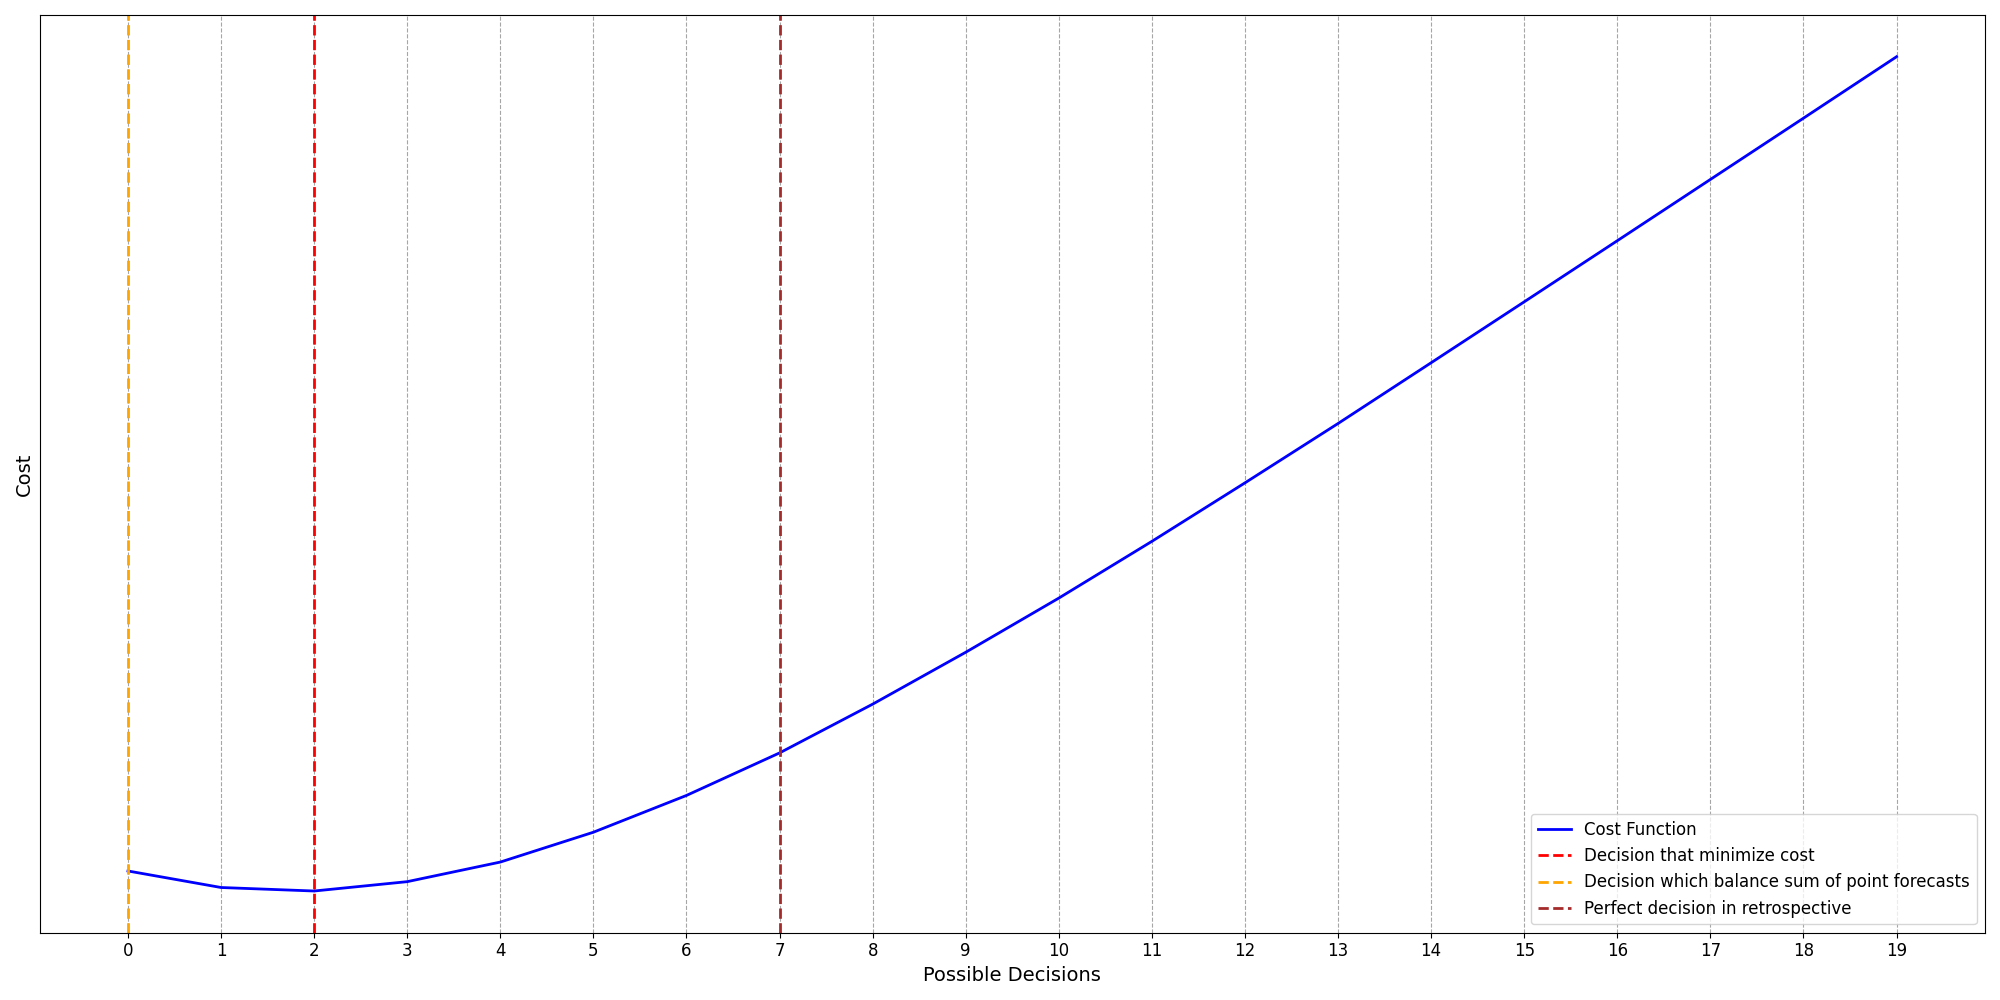
\includegraphics[width = 1\textwidth]{figures/cost_function.png}
		\caption{The figure show the decisions made from the decision rules of section \ref{sec:1} (yellow) and \ref{sec:2} (red) alongside the cost (blue) and the optimal decision in retrospective (brown).}
		\label{fig:cost_function}
	\end{figure} 
\end{example}

\section{Joint Probability}
Consider a system where $N_v$ vehicles, each carrying an unknown amount of units, are delivering units, and the number of units passing through a checkpoint per time step, denoted as $N_t$. Let the current time be denoted by $n$, then for $k$ steps into the future
\begin{equation}
	E[N_{n+k} |\{\tau\},I] = \sum_{N_{n+k}}N_{n+k}p(N_{n+k}|\{z\},I)
	\label{eq:E}	
\end{equation}
where $\{\tau\} = \{\tau^{(1)},\tau^{(2)},\dots\}$ is the set of travel times for each vehicle that has not yet arrived at the checkpoint and $I$ the background information and
\begin{equation}
	N_{n+k} = \sum_{i=1}^{N_v}N_{n+k}^{(i)}
	\label{eq:N}
\end{equation} 
with $N_{n+k}^{(i)}$ being the number of units delivered at time step $n+k$ by vehicle $i$. 
\begin{figure}[H]
	\centering
	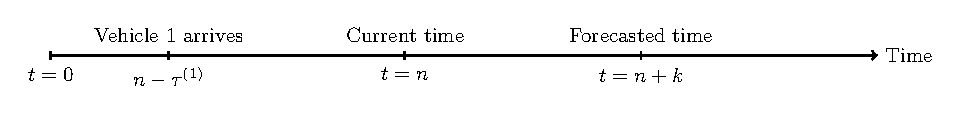
\includegraphics[width = 1\textwidth]{figures/vehicle_timeline.pdf}
	\caption{Timeline of vehicle arrivals.}
	\label{fig:vehicle_arrivals}
\end{figure}

Using \EQref{eq:N} in \EQref{eq:E}
\begin{equation}
	\begin{split}
		E[N_{n+k} |\{\tau\},I] &= \sum_{N_{n+k}^{(1)},N_{n+k}^{(2)},\dots}(N_{n+k}^{(1)}+N_{n+k}^{(2)}+\dots)p(N_{n+k}^{(1)},N_{n+k}^{(2)},\dots|\{z\},I)\\
		&=\sum_{i=1}^{N_v}\sum_{N_{n+k}^{(i)}} N_{n+k}^{(i)}p(N_{n+k}^{(i)}|z^{(i)},I)\\
		&=\sum_{i=1}^{N_v}\mathbb{E}[N_{n+k}^{(i)}|z^{(i)},I]\\
	\end{split}
	\label{eq:exp}
\end{equation}
where for the second equality it has been used that the vehicles are independent. Assuming the number of units for a given vehicle are Poisson (Poi) distributed with rate $\lambda^{(i)}$ 
\begin{equation}
	p(N_{n+k}^{(i)}|\tau^{(i)},I) = \text{Poi}(N_{n+k}^{(i)}|\lambda^{(i)},I)p(A|B),
	\label{eq:poi}
\end{equation}
where $A$ = "vehicle arriving at time step n+k" and $B$ = "the vehicle has not arrived at the checkpoint at time step n+k-1". From the chain rule
\begin{equation}
	\begin{split}
		p(A|B) &= \frac{P(A,B)}{P(B)}\\
		&= \frac{p(A)}{p(B)}
	\end{split}
	\label{eq:chain}
\end{equation}
where for the second equality it has been used that $p(A,B)=p(A)$ since $A$ can only happen if $B$ happens. Suppose the probability of arrival follows a negative binomial distribution (NB) with parameters $r, \theta$, then
\begin{equation}
	\begin{split}
		p(A) &= \text{NB}(\tau^{(i)}+k|r,\theta)\\
		p(B)& = 1-\sum_{t=1}^{\tau^{(i)}+k-1}\text{NB}(\tau^{(i)}+t|r,\theta).
	\end{split}
	\label{eq:neg_bin}
\end{equation}
Combining Equations \eqref{eq:exp}-\eqref{eq:neg_bin}
\begin{equation}
	\begin{split}
		E[N_{n+k} |\{\tau\},I] &=\sum_{i=1}^{N_v}\sum_{N_{n+k}^{(i)}} N_{n+k}^{(i)}\text{Poi}(N_{n+k}^{(i)}|\lambda^{(i)},I)\frac{\text{NB}(\tau^{(i)}+k|r,\theta)}{1-\sum_{t=1}^{\tau^{(i)}+k-1}\text{NB}(\tau^{(i)}+t|r,\theta)}\\
		&=\sum_{i=1}^{N_v}\lambda^{(i)}\frac{\text{NB}(\tau^{(i)}+k|r,\theta)}{1-\sum_{t=1}^{\tau^{(i)}+k-1}\text{NB}(t|r,\theta)}\\
	\end{split}
\end{equation}


NOTE: Next up I want to expand the model to include data from i) past travel times and past number of units carried by vehicles. This data should be used to learn parameters $\lambda^{(i)}$ and $r,\theta$.

I want to make a pymc model. In that case I would assign $\lambda^{(i)},r,\theta$ priors: Gamma,  Poi, Beta.